\chapter{Blockchain Technology} \label{ch:blockchain}

In the current landscape, blockchain technology has attracted increasing global interest due to its promising applications and potential transformative impacts on various 
sectors. Founded in 2008 by Satoshi Nakamoto as the mainstay of the Bitcoin system \cite{9752154}, blockchain has evolved from a simple ledger of financial transactions 
to a fundamental technology that revolutionizes the way information is recorded, shared and managed within decentralized networks.

\section{What is the Blockchain}

The blockchain is a core technology that drives many decentralized systems offering transparency, trust and safety without having to have a central authority. It is 
basically a distributed ledger that operates through the peer-to-peer \cite{9596538}, \cite{ibm_blockchain}. This section talks of the key components and architecture in 
blockchain, revealing its fundamental features and operating principles.

\subsection{Core Elements of Blockchain}

The blockchain comprises several key elements essential to its functionality:

\begin{itemize}
  \item \textbf{Blocks}: A block is a basic unit comprising of transactional data. Every block is securely connected to the previous one; this connection creates a chain 
  of blocks. The transactions within a block are cryptographically secured; hence, immutability and integrity \cite{9596538}, \cite{ibm_blockchain}.
  \item \textbf{Transactions}: Transactions are diverse interactions in the blockchain network. These interactions are not limited to the financial transfers only; any 
  piece of valuable information can be considered as a transaction and diffused within the network \cite{9752154}, \cite{9036241}.
  \item \textbf{Decentralization}: Unlike centralized systems that depend on a single controlling authority, the blockchain is decentralized. It includes a web of 
  interdependent nodes, each replicating the distributed registry. Resilience, transparency and no single points of failure are guaranteed by decentralization \cite{9596538}, \cite{9752154}.
  \item \textbf{Consensus Mechanism}:  For verification and agreement of the state of a ledger, blockchain uses consensus mechanisms. The most common mechanism, \gls{pow}, 
  requires miners to solve the complicated cryptographic puzzles in order to add new blocks on the chain. Consensus mechanisms ensure consensus among network participants 
  to prevent attacks by malicious actors \cite{9596538}, \cite{9752154}.
\end{itemize}

\subsection{Blockchain Architecture}

The structure of the system is carefully crafted to uphold its principles of decentralization, immutability and transparency;

\begin{itemize}
  \item \textbf{\gls{dlt}}: At the core of blockchain lies DLT, where all participants, in the network have access to a ledger of transactions. 
  This shared ledger eliminates redundancy. Ensures that everyone has a trusted source of information across the network \cite{ibm_blockchain}, \cite{9752154}.
  \item \textbf{Immutable Records}: One key feature of blockchain is its records immutability. Once a transaction is recorded on the ledger it cannot be. Tampered with. 
  Any attempt to change a transaction requires adding an one preserving the integrity of data \cite{ibm_blockchain}.
  \item \textbf{Smart Contracts}: Smart contracts are self executing contracts with predefined rules embedded within the blockchain. These contracts. Enforce agreements 
  between parties speeding up transaction processing and reducing reliance on intermediaries \cite{ibm_blockchain}, \cite{9036241}.
  \item \textbf{Security Measures}:  Cryptography plays a role in ensuring security by protecting transactions from tampering and fraud. Private key pairs authenticate. 
  Enable secure digital identity management. Additionally cryptographic hashing guarantees data integrity and confidentiality \cite{9596538}, \cite{9036241}.
  \item \textbf{Peer-to-Peer Network}: The blockchain functions using a network architecture where participants can directly communicate and interact. This decentralized 
  structure promotes trust and resilience since transactions are verified and validated through consensus, among distributed nodes \cite{9752154}, \cite{9036241}.
\end{itemize}

\begin{figure}[h]  
  \centering
  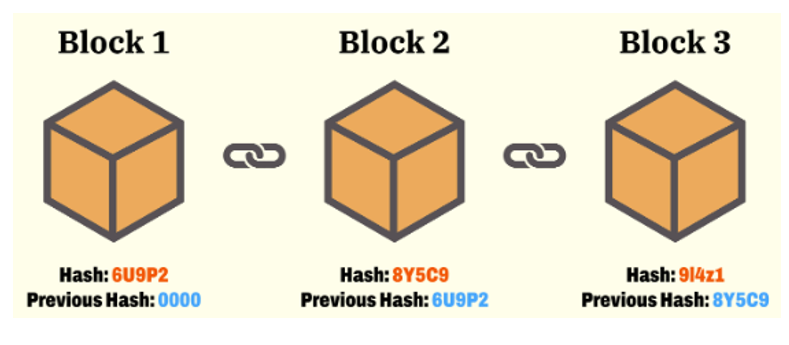
\includegraphics[width=0.7\textwidth]{Images/c2_1.png} 
  \caption{Blockchain structure}
\end{figure}

\section{How the Blockchain works}

The function of a blockchain system encompasses a complex chain of procedures that safeguard the  integrity, transparency, and security of transactions. In this section, 
we delve into the fundamental mechanisms of blockchain.

\subsection{Transaction process}

\subsubsection{Recording transactions}

\begin{enumerate}
    \item \textbf{Starting a Transaction:} In a network, users initiate transactions through their wallets. Each wallet has a pair of keys. A key, for starting transactions 
    and a private key for authentication \cite{9596538}.
    \item \textbf{Creating Blocks:} As transactions take place they are grouped together into blocks of data. These blocks act as containers for recording details like 
    asset movement participants involved and timestamps \cite{ibm_blockchain}.
    \item \textbf{Hashing:} Every block contains information and refers to the hash of the previous block. Secure hash functions like SHA 256 play a role in ensuring the 
    integrity and immutability of transactions. Hashing allows each block to have a fingerprint making identification and verification simple \cite{ibm_blockchain} ,\cite{9036241}.
\end{enumerate}

\subsubsection{Consensus Mechanism}

\begin{enumerate}
    \setcounter{enumi}{3}
    \item \textbf{Verification Process:} When a transaction is initiated the information is sent to a network of distributed peer, to peer nodes. These nodes work together 
    to confirm the validity of transactions using consensus mechanisms \cite{9036241}, \cite{geeksforgeeks}.
    \item \textbf{Formation of New Blocks:} Valid transactions are added to a \gls{mempool} where they wait to be included in a block. Miners, who are responsible 
    for creating blocks solve cryptographic puzzles in order to mine blocks. This process, known as \gls{pow} requires resources and time \cite{9596538}, \cite{geeksforgeeks}.
    \item \textbf{Consensus Algorithm:} In order to add a block to the blockchain nodes must agree on its validity through consensus algorithms. The miner who successfully 
    creates a block is rewarded. Consensus algorithms ensure that all nodes are synchronized and in agreement, about the state of the blockchain \cite{geeksforgeeks}.
    \item \textbf{Blockchain Integrity:} The interconnected nature of blocks ensures the immutability and integrity of the blockchain. Each block references the hash value 
    of its predecessor making it practically impossible to tamper with transactions without altering blocks \cite{9596538} ,\cite{9036241}.
\end{enumerate}

\begin{figure}[h]  
  \centering
  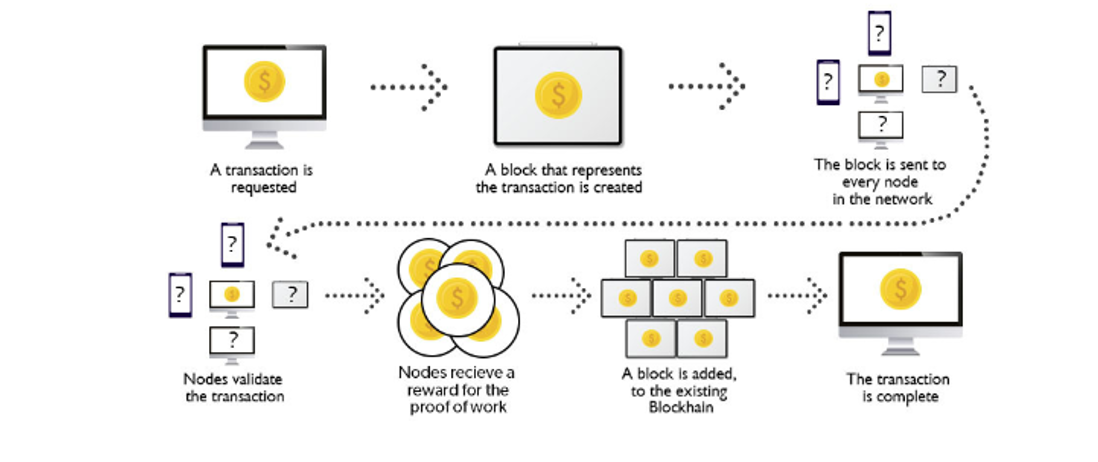
\includegraphics[width=1\textwidth]{Images/c2_2.png} 
  \caption{Blockchain transaction process}
\end{figure}

\subsection{Blockchain Benefits}

Due to the execution process described above and its architecture, blockchain is able to offer many benefits in different areas:

\begin{itemize}
  \item \textbf{Greater Trust:} Blockchain helps establish trust across the network through utilizing the decentralized ledger, making sure that data is consistent and 
  timely plus, it doesn’t require intermediaries \cite{9596538}. 
  \item \textbf{Enhanced Security:} Blockchain's security features are designed to thwart tampering as well as cybercrime. The blockchain structures transactions as 
  read-only data which is difficult to change and ensures that the data is protected even when it is in transit. Moreover, cryptography is used as a mechanism of 
  verification and the cryptographic infrastructure is used to store and transmit secrets \cite{ibm_blockchain}.
  \item \textbf{Time Savings:} The utilization of blockchain technology decreases greatly the processing time for transactions since they get completed within a quarter of 
  an hour due to the removal of the centralized authority that confirms \cite{ibm_blockchain}.
  \item \textbf{Cost Savings:} The blockchain adjusts transaction procedure and lowers operational costs by the removal of intermediaries, as tasks are automated and there 
  is lower duplication of activities through the usage of shared ledger \cite{9596538}, \cite{9036241}.
  \item \textbf{Efficiency Improvements:} The distributed architecture of blockchain increases system resilience, decreases processing costs, and removes the need for 
  centralized network control by distributing network operations thinly, facilitating faster settlements, and solving identity management issues \cite{9036241}.
  \item \textbf{Transparency Enhancement:} A blockchain keeps a permanent record of transactions through which it delivers transparency, accountability and trust to the 
  network users via its chronological and transparent nature \cite{9036241}.
\end{itemize}

\section{Blockchain Classification}

\subsection{Types of Blockchains}

The blockchain technology comes in various forms, each with unique characteristics that adapt to specific needs and application contexts Beyond the well-known public and 
private blockchains, it's essential to recognize two other significant variants: hybrid chains and consortium chains.

\newpage

\begin{itemize}
  \item \textbf{Public Blockchain:} A public blockchain is open to everybody who wants to interact and contribute to the consensus protocol, e.g., Bitcoin. 
  This model provides a high degree of transparency though, it is susceptible to 51\% attacks. Its open nature fosters a distrustful environment, as no one individual or 
  entity is solely relied on for transaction validation \cite{9596538}, \cite{ibm_blockchain}.
  \item \textbf{Private Blockchain:} In contrast to public blockchains, private or permissioned (access is restricted to authorized entities) blockchains 
  allow only a limited set of entities to access the network. This method is popular among situations that demand more of such features such as security as well as control 
  where it gets applied in applications like financial transactions that also handle sensitive data. An access to the network is controlled by a single entity or by 
  particular criteria \cite{9596538},\cite{9036241}.
 \item \textbf{Consortium Blockchain:} A consortium blockchain is governed by more than one organization or entity working together to ensure the distributed ledger. 
  On the other hand, blockchains that are public or private, consortium blockchains are the only ones that give power to a chosen group of nodes to validate and record 
  transactions. This model is suitable where several subjects need to work with data and processes together but they do not want or they cannot fully trust a unique 
  central entity \cite{ibm_blockchain}, \cite{9752154}.
\end{itemize}

\renewcommand{\arraystretch}{1.3}
\begin{table}[h]
  \centering
  \begin{tabularx}{\textwidth}{|>{\centering\arraybackslash}m{3.2cm}|>{\centering\arraybackslash}m{3.2cm}|>{\centering\arraybackslash}m{3.4cm}|>{\centering\arraybackslash}m{3.2cm}|}
    \hline
    \thead{Property} & \thead{Public \\ Blockchain} & \thead{Consortium \\ Blockchain}  & \thead{Private \\ Blockchain} \\
    \hline
    Consensus determination & All miners & Selected set of nodes  & One organization \\
    \hline
    Read permission & Public & Could be public or restricted & Could be public or restricted \\
    \hline
    Efficiency & Low & High & High \\
    \hline
    Immutability & Nearly impossible to transfer & Could be tampered & Could be tampered \\
    \hline
    Centralized & No & Partial & Yes \\
    \hline
    Consensus process & Permissionless & Permissioned & Permissioned \\
    \hline
  \end{tabularx}
  \caption{Types of Blockchain}
\end{table}

\newpage

\begin{itemize}
  \item \textbf{Hybrid Blockchain:} In addition to the previous ones mentioned above, a new type of blockchain, hybrid blockchains, has also emerged. They are described by the property of switching between different modes having different types of 
  operating systems, for example, public and private blockchains that suit specific needs. This approach provides a greater degree of flexibility and customization compared 
  to conventional blockchain configurations; thereby, the actors have the option to decide the degree of decentralization and control that is suitable for them \cite{9596538}.
\end{itemize}

\subsection{Types of Consensus Mechanisms}

Blockchains also differ based on the type of consensus mechanism used. In the previous section we discussed an example of how blockchain uses a consensus mechanism called 
\gls{pow} \cite{9752154}, \cite{10037907}. However there are several types of consensus mechanisms that can be used in a blockchain network. 

In general, the two main types of consensus mechanisms are: \gls{pow} and \gls{pos}. With \gls{pow} miners solve puzzles to add new blocks, which requires significant 
computational resources and time \cite{9752154}, \cite{10037907}. This is elaborated further in Section \ref{subsec:bitcoin}. On the hand \gls{pos} assigns the right 
to create blocks based on participants cryptocurrency holdings providing benefits such, as energy efficiency and scalability advantages. Further information,
about PoS can be found in Section \ref{subsec:ethereum}. There are also other consensus mechanisms beyond \gls{pow} and \gls{pos}; refer to the table for further details.

\renewcommand{\arraystretch}{1.3}
\begin{table}[h]
  \centering
  \begin{tabularx}{\textwidth}{|>{\centering\arraybackslash}m{2.4cm}|>{\centering\arraybackslash}m{1.8cm}|>{\centering\arraybackslash}m{1.9cm}|>{\centering\arraybackslash}m{2.3cm}|>{\centering\arraybackslash}m{1.9cm}|>{\centering\arraybackslash}m{1.8cm}|}
    \hline
    \thead{Property} & \thead{PoW} & \thead{PoS}  & \thead{PBFT} & \thead{DPOS} & \thead{Ripple} \\
    \hline
    Node identity management & Open & Open & Permissioned & Open & Open \\
    \hline
    Energy saving & No & Partial & Yes & Partial & Yes  \\
    \hline
    Tolerated power of adversary & $<$25\% computing power & $<$51\% stake & $<$33.3\% faulty replicas & $<$51\% validators & $<$20\% faulty nodes in UNL  \\
    \hline
    Example & Bitcoin & Ethereum & Hyperledger Fabric & Bitshares & Ripple  \\
    \hline
  \end{tabularx}
  \caption{Types of Consensus Mechanism}
\end{table}


\section{Bitcoin versus Ethereum}

Bitcoin and Ethereum stand as two big giants in the blockchain technology area, and both of them possess their own characteristics and they make their own contributions to the ever-changing world of decentralized systems.
This section takes a comparative approach between Bitcoin and Ethereum; analyzing their basic architectures, transaction mechanisms, consensus methods, cryptographic techniques, and what advantages and lacks they can offer.

\subsection{Bitcoin} \label{subsec:bitcoin}

\subsubsection{Overview}

Bitcoin, launched in 2008 by Satoshi Nakamoto, is a decentralized digital currency that is also accompanied by the great invention, the blockchain. It functions as a 
peer-to-peer decentralized electronic payment system; it introduces a new way of executing business transactions and the security of data \cite{9129332}. Bitcoin is an open-source 
and permissionless blockchain, allowing for involvement of anyone with the required hardware.

\subsubsection{Transaction mechanism}

When a user sends bitcoins, sender hashed addresses, recipient hashed addresses, transaction amount and fee. Digital signatures prove property rights and the transaction 
is floated to the network, being submitted to the mempool for confirmation \cite{bitcoincom}. The mining being the process of validating transactions and so the miners pick transactions 
from the \gls{mempool} in order to create new blocks by solving complex mathematical puzzles called \gls{pow} \cite{9129332}. The winner of the puzzle then 
broadcasts their newly found block to the network. After a verification done by other network nodes, the block is added to the blockchain, thus finalizing the transaction.

\subsubsection{Proof of Work}

Bitcoin uses the \gls{pow} consensus algorithm to maintain agreement among network participants about the validity of transactions. The \gls{pow} was first 
specified in the Hashcash paper \cite{9129332}. It requires the miners to search solutions of cryptographic puzzles consuming computational power. Through the cost of computation, the miners
establish their commitment to the security of the network as changing the blockchain will require enormous computational resources, hence, making fraudulent endeavors expensive.

\subsubsection{Bitcoin Cryptography}

Bitcoin use the \gls{sha2} for cryptographic hashing, which ensures irreversible and collision resistive attributes. This guarantees the data integrity of the 
blockchain, which makes it impractical to tamper with transactions that are already in the database. Moreover, the Merkle Trees that Bitcoin natively uses for block data 
encoding take security to the next level \cite{9129332}.

\subsubsection{Unspent Transaction Output} 

Bitcoin transactions are registered in the blockchain as \gls{utxo}s, which meaning constant fractions of bitcoins that are linked to certain owner. 
This \gls{utxo} is pervasively distributed over the blockchain and represents ownership. It is subsequently used in other transactions too. Bitcoin balances are not stored in user 
accounts but rather tracked through the \gls{utxo}s associated with their addresses \cite{bitcoincom}.

\begin{figure}[h]  
  \centering
  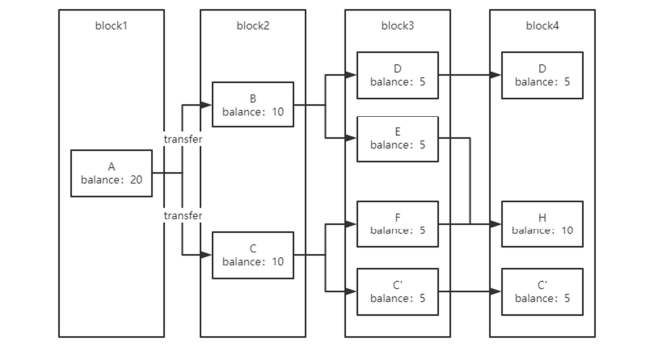
\includegraphics[width=0.7\textwidth]{Images/c2_3.png} 
  \caption{UTXO transaction process}
\end{figure}

\subsubsection{Advantages and Limitations}

Bitcoin is decentralized and provides encryption security that can be used to resist censorship, to ensure accessibility particularly on a global scale and to preserve integrity 
of the data. Nevertheless, Bitcoin has such limitations as scalability problem, transaction throughput rate without the corresponding increase in the number of transactions 
and undulatory acceptance and valuation. Furthermore, there are additional security concerns, such as the "51\% attack" and human error, which continue to plague the Bitcoin 
ecosystem \cite{9129332}.

\subsection{Ethereum} \label{subsec:ethereum}

\subsubsection{Overview}

Ethereum, designed by Vitalik Buterin, is the introduction of Smart Contracts to the crypto-sphere, which is a novelty in the blockchain space, and, obviously, it has been 
a highly valuable addition. The September 2022 saw the newly born Ethereum 2.0 replace Ethereum 1.0 by incorporating the Beacon Chain and the shift from \gls{pow} 
to \gls{pos} consensus mechanism \cite{ethereummerge}. This change shall constitute one of the really important milestones reached by Ethereum, the blockchain providing 
scalability, sustainability, as well as security.

\subsubsection{Beacon Chain Impact}

The introduction of the Beacon Chain revolutionized Ethereum's operating model \cite{ethereummerge}. It replaced the original execution layer (Mainnet) and introduced a new consensus layer, 
the \gls{pos} which was a major improvement in terms of power consumption and the amount of energy consumed reduced from 99.95\%. Validators, staking their ETH, assumed the 
responsibility of block production and transaction validation, moving away from energy-intensive mining. This transition helped create a sustainable network 
architecture as well as secure the information connections.

\subsubsection{Transaction Mechanism}

In Ethereum 2.0, validators play a pivotal role by depositing 32 ETH and operating three essential software components: a execution client, a client for consensus, and a client for 
validation as well. Here we have the validators appointed randomly for being picked on 12 second timeslots which then make up epochs composed of 32 slots. They formulate 
and verify blocks and this way they add to the Ethereum System. This process regulates all the transactions on the blockchain. Transactions include processing stages of 
creating, verifying, and block proposal irrespective of the fact that the transactions are created, verified, combined into execution payloads, and broadcasted across 
the network so as to make self-enforcement and fault-tolerance in proper working order. Finality being one of the main features of transaction irreversibility, is 
sealed by using checkpoints that initiate even the smallest epochs. As requisite effort to checkpoints pairs, validators vote in a supermajority to revert them, 
consequently, block reversal is discouraged and the entire Ethereum network is protected from brainwashing attacks \cite{ethereumpos}.

\subsubsection{Proof of Stake}

The Ethereum 2.0 version puts the \gls{pos} consensus mechanism at the core of the protocol with validators given the chance to make the most of their 
investment through staking \cite{ethereumpos}. Validator's deposit their own ETH as bond to release validator software which helps in the job of validating the transactions and 
generating new blocks proposals. In contrast to proof-of-work, the \gls{pos} is doing well in maintaining both the security and the decentralization of validators that 
attempt to undermine the network due to its feature of penalization.

\begin{figure}[h]  
  \centering
  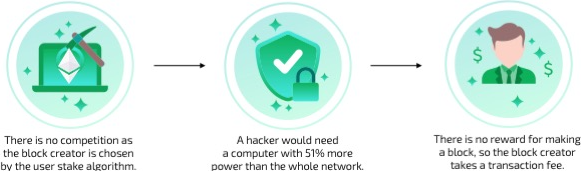
\includegraphics[width=1\textwidth]{Images/Cattura.PNG} 
  \caption{Ethereum Proof of Stake's features.}
\end{figure}

\subsubsection{Ethereum Cryptography}

Ethereum 2.0 still relies heavily on the standards of crypto- security for safety, keeping the Keccak-256 algorithm implemented by Ethereum 1.0. These 
algorithmic primitives give Ethereum strong security by making sure the data integrity, confidentiality, and authenticity \cite{9129332}.

\subsubsection{Advantages and Limitations}

The new Ethereum 2.0 version has several new advantages. The transition from \gls{pow} to \gls{pos} results in a substantial reduction in energy and makes Ethereum more sustainable. In 
addition, the \gls{pos} model makes the network more secure, decentralized and scalable, so that a thriving ecosystem of decentralized applications can grow within it \cite{ethereumpos}. 
However, even this version, still has some drawbacks. Processing time can still be a bottleneck, as Ethereum cannot process transactions at the same speed as traditional 
processes, such as Visa \cite{9129332}. Besides, market fluctuations and rumors become the main problems for Ethereum's stability and reputation, which requires continuous 
technological development and management.
